% For printing purposes only
%\documentclass[8pt,handout]{beamer}
%\usepackage{pgf,pgfpages}
%\usepackage{handoutWithNotes}
%\pgfpagesuselayout{4 on 1 with notes}[letterpaper,border shrink=5mm,portrait]


\documentclass[smaller,compress,mathserif]{beamer}
\usepackage{mybeamertheme_light}

\usepackage{multimedia} % to embed movies in the PDF file
\usepackage{graphicx}
\usepackage{comment}
\usepackage[english]{babel}
\usepackage{amsmath}
\usepackage{amsfonts}
\usepackage{subfigure}
\usepackage{wrapfig}
\usepackage{multirow}
\usepackage{algorithmic}
\usepackage[ruled,vlined]{algorithm2e}
\usepackage{tikz}

\setbeamertemplate{bibliography item}{\insertbiblabel}

%%%% Images
\pgfdeclareimage[height=0.8cm]{ricelogoimage}{rice_logo}

%%%% Math macros
%!TEX root = main.tex



\newcommand{\eref}[1]{\mbox{\rm(\ref{#1})}}
\newcommand{\tref}[1]{\mbox{\rm\ref{#1}}}
\newcommand{\set}[2]{\left\{ #1 \; : \; #2 \right\} }
\newcommand{\deq}{\raisebox{0pt}[1ex][0pt]{$\stackrel{\scriptscriptstyle{\rm def}}{{}={}}$}}

\newcommand {\DS} {\displaystyle}

\newcommand{\real}{\mathbb{R}}



\newcommand {\half} {\mbox{$\frac{1}{2}$}}
\newcommand{\force}{{\mathbf{f}}}
\newcommand{\strain}{{\boldsymbol{\varepsilon}}}
\newcommand{\stress}{{\boldsymbol{\sigma}}}
\renewcommand{\div}{{\boldsymbol{\nabla}}}

\newcommand {\cA} {{\cal A}}
\newcommand {\cB} {{\cal B}}
\newcommand {\cC} {{\cal C}}
\newcommand {\cD} {{\cal D}}
\newcommand {\cE} {{\cal E}}
\newcommand {\cK} {{\cal K}}
\newcommand {\cL} {{\cal L}}
\newcommand {\cP} {{\cal P}}
\newcommand {\cQ} {{\cal Q}}
\newcommand {\cR} {{\cal R}}
\newcommand {\cV} {{\cal V}}
\newcommand {\cW} {{\cal W}}
\newcommand {\CC} {{\cal C}}
\newcommand {\CD} {{\cal D}}
\newcommand {\CH} {{\cal H}}
\newcommand {\CS} {{\cal S}}
\newcommand {\CU} {{\cal U}}
\newcommand {\CY} {{\cal Y}}



\newcommand{\bzero}{\mathbf{0}}
\newcommand{\ba}{\mathbf{a}}
\newcommand{\bb}{\mathbf{b}}
\newcommand{\bc}{\mathbf{c}}
\newcommand{\bd}{\mathbf{d}}
\newcommand{\be}{\mathbf{e}}
\newcommand{\bg}{\mathbf{g}}
\newcommand{\bh}{\mathbf{h}}
\newcommand{\bl}{\mathbf{l}}
\newcommand{\bn}{\mathbf{n}}
\newcommand{\bp}{\mathbf{p}}
\newcommand{\bq}{\mathbf{q}}
\newcommand{\br}{\mathbf{r}}
\newcommand{\bs}{\mathbf{s}}
\newcommand{\bt}{\mathbf{t}}
\newcommand{\bu}{\mathbf{u}}
\newcommand{\bv}{\mathbf{v}}
\newcommand{\bw}{\mathbf{w}}
\newcommand{\bx}{\mathbf{x}}
\newcommand{\by}{\mathbf{y}}
\newcommand{\bz}{\mathbf{z}}
\newcommand{\bA}{{\mathbf A}}
\newcommand{\bB}{\mathbf{B}}
\newcommand{\bC}{\mathbf{C}}
\newcommand{\bD}{\mathbf{D}}
\newcommand{\bE}{\mathbf{E}}
\newcommand{\bF}{\mathbf{F}}
\newcommand{\bG}{\mathbf{G}}
\newcommand{\bH}{\mathbf{H}}
\newcommand{\bI}{\mathbf{I}}
\newcommand{\bJ}{\mathbf{J}}
\newcommand{\bK}{\mathbf{K}}
\newcommand{\bL}{\mathbf{L}}
\newcommand{\bM}{\mathbf{M}}
\newcommand{\bN}{\mathbf{N}}
\newcommand{\bO}{\mathbf{O}}
\newcommand{\bP}{\mathbf{P}}
\newcommand{\bQ}{\mathbf{Q}}
\newcommand{\bR}{\mathbf{R}}
\newcommand{\bS}{\mathbf{S}}
\newcommand{\bU}{\mathbf{U}}
\newcommand{\bV}{\mathbf{V}}
\newcommand{\bW}{\mathbf{W}}
\newcommand{\bX}{\mathbf{X}}
\newcommand{\bY}{\mathbf{Y}}
\newcommand{\bZ}{\mathbf{Z}}

\newcommand{\bgamma}{{\boldsymbol{\gamma}}}
\newcommand{\bmu}{{\boldsymbol{\mu}}}
\newcommand{\bkappa}{{\boldsymbol{\kappa}}}
\newcommand{\blambda}{{\boldsymbol{\lambda}}}
\newcommand{\bLambda}{{\boldsymbol{\Lambda}}}
\newcommand{\bpi}{{\boldsymbol{\pi}}}
\newcommand{\bPi}{{\boldsymbol{\Pi}}}
\newcommand{\btheta}{{\boldsymbol{\theta}}}
\newcommand{\bTheta}{{\boldsymbol{\Theta}}}
\newcommand{\bSigma}{{\boldsymbol{\Sigma}}}






\newcommand{\red}{\color[rgb]{0.6,0,0}}
\newcommand{\green}{\color[rgb]{0,0.6,0}}
\newcommand{\blue}{\color[rgb]{0,0,0.6}}
\newcommand{\darkgreen}{\color[rgb]{0,0.6,0}}
\newcommand{\lightgray}{\color[rgb]{0.5,0.5,0.5}}
\newcommand{\magenta}{\color[rgb]{0.7,0.0,0.5}}



\definecolor{navy}{RGB}{0,0,128}
\definecolor{forestgreen}{RGB}{34,139,34}
\definecolor{darkred}{RGB}{128,0,0}
\definecolor{mylightsteelblue}{RGB}{176,196,222}
\definecolor{mylightcyan}{RGB}{180,255,255}
\definecolor{mypaleturquoise}{RGB}{175,238,238}
\definecolor{mylightgoldenrod}{RGB}{250,250,210}
\definecolor{mylightyellow}{RGB}{255,255,224}
\definecolor{mylightsalmon}{RGB}{255,160,122}

\setbeamercolor{blacklightsteelblue}{fg=black,bg=mylightsteelblue}
\setbeamercolor{blackpaleturquoise}{fg=black,bg=mypaleturquoise}
\setbeamercolor{blacklightcyan}{fg=black,bg=mylightcyan}
\setbeamercolor{blacklightgoldenrod}{fg=black,bg=mylightgoldenrod}
\setbeamercolor{blacklightyellow}{fg=black,bg=mylightyellow}
\setbeamercolor{blacklightsalmon}{fg=black,bg=mylightsalmon}
\setbeamercolor{blackcyan}{fg=black,bg=cyan}




%%%%%%%%%%%%%%%%%%%%%%%%%%%%%%%%%%%%%%%%%%%%%%%%%%%%%%%%%%%%%%%%%%%%%%%%%%
%%% Title Page %%%%%%%%%%%%%%%%%%%%%%%%%%%%%%%%%%%%%%%%%%%%%%%%%%%%%%%%%%%
%%%%%%%%%%%%%%%%%%%%%%%%%%%%%%%%%%%%%%%%%%%%%%%%%%%%%%%%%%%%%%%%%%%%%%%%%%

\title{ {\Large \bf Data Driven Model Reduction for Linear Time-Invariant Dynamical Systems}}

\author[Mark Kessler and Alex Bluestein]{Mark Kessler and Alex Bluestein}
\institute[Rice University]
{Department of Computational and Applied Mathematics \\
    Rice University, Houston, Texas \\
\texttt{mak17@rice.edu, arb19@rice.edu}}
\date[June \& July, 2019]{June \& July, 2019}



%\AtBeginSubsection[]
%{
%  \begin{frame}<beamer>
%    \frametitle{Outline}
%    \tableofcontents[currentsection,currentsubsection]
%    \end{frame}
%}

\AtBeginSection[]
{
  \begin{frame}<beamer>
    \frametitle{Outline}
    \tableofcontents[currentsection]
  \end{frame}
}


\begin{document}



\begin{frame}
  \titlepage
  
  \begin{center}
    REU Summer 2019\\[2ex]
 \end{center}
 
 \end{frame}

%%%%%%%%%%%%%%%%%%%%%%%%%%%%%%%%%%%%%%%%%%%%%%%%%%%%%%%%%%%%%%%%%%%%%%%%%%
%%% Presentation Body %%%%%%%%%%%%%%%%%%%%%%%%%%%%%%%%%%%%%%%%%%%%%%%%%%%%
%%%%%%%%%%%%%%%%%%%%%%%%%%%%%%%%%%%%%%%%%%%%%%%%%%%%%%%%%%%%%%%%%%%%%%%%%%



%\include{fem}



\section{Introduction}

\begin{frame}{Problem}
Given\\
\bigskip
$\bA, {\bf E} \in \real^{n \times n}$, ${\bf B} \in \real^{n \times m}$, ${\bf C} \in \real^{k \times n}$, and ${\bf D} \in \real^{k \times m}$\\
\bigskip
consider a system with $m$ inputs and $k$ outputs of the type:
\begin{align*}
            {\bf E}\frac{d}{dt} {\bf y}(t)  &= \bA {\bf y}(t) + {\bf B}{\bf u}(t)\\
            {\bf z}(t) &= {\bf C} {\bf y}(t) + {\bf D}{\bf u}(t)
\end{align*}

with n large (\(>1000\)). !!Expensive to solve!!
\bigskip

Goal - Create a reduced order model\\
\bigskip
$\widehat \bA, {\bf \widehat E} \in \real^{r \times r}$, ${\bf \widehat B} \in \real^{r \times m}$, ${\bf \widehat C} \in \real^{k \times r}$, and ${\bf \widehat D} \in \real^{k \times m}$\\
\bigskip
with r small (\(<20\)) that approximates the original model


\end{frame}

%%%%%%%%%%%%

\begin{frame}{Reduced Order Model Techniques}

Our research focuses on:
\bigskip
    \begin{itemize}
        \item <1-> Interpolatory techniques
        \begin{itemize}
            \item <1-> Projection Based
            \item <1-> Loewner Method
        \end{itemize}
    \end{itemize}
    \bigskip
    Each technique will require working in frequency space.\\
    \bigskip
    To operate in frequency space, we must apply the Laplace Transform to the time-dependent system.
\end{frame}
\section{1D Time-Dependent Advection Diffusion Equation}

\begin{frame}{1D Time-Dependent Advection Diffusion Equation}
	Partial differential equation (PDE):
	 \begin{align*}
                         \frac{\partial}{\partial t} y(x,t) 
                        - \alpha \frac{\partial^2}{\partial x^2} y(x,t) +  \beta \frac{\partial}{\partial x} y(x,t) &= 0
                                                & x \in (0,1), t \in (0,T), \\
                         y(0,t) &= u(t),    & t \in (0,T), \\
                         y_x(1,t) &= 0,    & t \in (0,T), \\
                         y(x,0) &= y_0(x),  & x \in (0,1),
          \end{align*}
          with $\alpha > 0$ and $\beta >0$. We use
         \[
                \alpha=0.01, \beta = 1, T=0.5.
          \]
        \begin{minipage}[c]{0.6\textwidth}
	Output:
	\[
	   z(t) = \int_{0}^{1} y(x,t) dx
	\]
	\end{minipage} \hfil
         \begin{minipage}[c]{0.35\textwidth}
	\begin{center}
               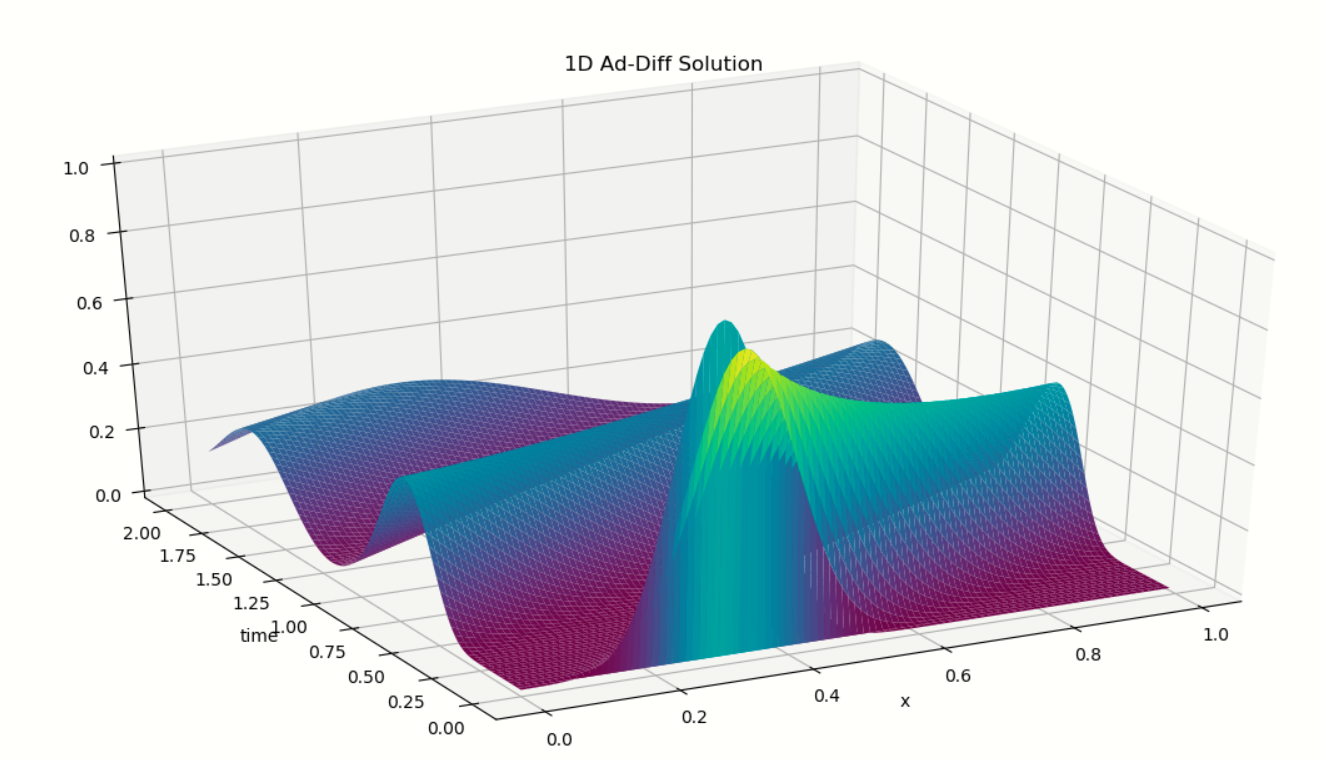
\includegraphics[width=1.0\textwidth]{figures/1D_addiffsol.PNG}\\
               PDE solution
	\end{center}
	\end{minipage}
\end{frame}
%%%%%%%%%%%%%%%%%%%%%%%%%%%%%%%%%%%%%%%%%%
\begin{frame}{SISO Notation}
Proposed system is single input (${\bf u}(t) \in \real$) and single output (${\bf z}(t) \in \real$)\\
\bigskip
Change of notation:\\
\bigskip
$\bA, {\bf E} \in \real^{n \times n}$, ${\bf b},{\bf c} \in \real^n$, and ${\bf d} \in \real$\\

\begin{align*}
            {\bf E}\frac{d}{dt} {\bf y}(t)  &= \bA {\bf y}(t) + {\bf b}{\bf u}(t)\\
            {\bf z}(t) &= {\bf c}^T {\bf y}(t) + {\bf d}{\bf u}(t)
\end{align*}


\end{frame}


%%%%%%%%%%%%%%%%%%%%%%%%%%%%%%%%%%%%%%%%%%%%%%%%%%%%%%%%%%%%%%%%%%%%%%%%%%

\begin{frame}{1D Advection Diffusion Discretization}

Upwind finite difference discretization in space leads to
         \[
                    \frac{d}{dt} {\bf y}(t)  = \bA {\bf y}(t) + {\bf b}{\bf u}(t), \quad t \in (0,T), \qquad {\bf y}(0) = {\bf y}_0,
        \]
        where \({\bf A} = \alpha \bA^{diff} + \beta \bA^{conv}\)
        \begin{align*}
              \setlength{\arraycolsep}{2pt}
              \renewcommand{\arraystretch}{0.9}
              \bA^{diff} = \begin{bmatrix}
              -2 & 1\\
              1 & -2 & -1\\
              &   \ddots & \ddots & \ddots\\
              &   &     1 & -2 & 1\\
              &&& 2 & -2
              \end{bmatrix}
        &
              \setlength{\arraycolsep}{2pt}
              \renewcommand{\arraystretch}{0.9}
              \bA^{conv} = \begin{bmatrix}
              -1\\
              1 & -1 \\
              &   \ddots & \ddots\\
              &   &     1 & -1\\
              &&& 1 & -1
              \end{bmatrix}
        \end{align*}
        \[
             {\bf y}_0 =  \Big(y_0(x_0,t), \ldots,  y_0(x_{n_x-1},t) \Big)^T \in \real^{n_x}             
        \]
        
        \[
             {\bf b} =  \Big( \frac{\alpha}{h^{2}}+\frac{\beta}{h},0, \ldots,0 \Big)^T \in \real^{n_x}             
        \]

\end{frame}


%%%%%%%%%%%%%%%%%%%%%%%%%%%%%%%%%%%%%%%%%%%%%%%%%%%%%%%%%%%%%%%%%%%%%%%%%%%%%%%%%%%%

\begin{frame}{1D Advection Diffusion Discretization (cont.)}

Composite Trapezoidal Rule:
\begin{align*}
     \int_{0}^{1} y(x,t)dx & \approx \frac{h}{2} y(x_0,t) + hy(x_1,t) + \ldots + hy(x_{n_x -1},t) + \frac{h}{2} y(x_n,t)
     \\
     & = \frac{h}{2}u(t) + hy(x_1,t) + \ldots + hy(x_{n_x -1},t) + \frac{h}{2} y(x_n,t)\\
\end{align*}
    
Leads to:
\begin{align*}
     \int_{0}^{1} y(x,t)dx & \approx \frac{h}{2} u(t) + hy_1(t) + \ldots + hy_{n_x -1}(t) + \frac{h}{2} y_{n_x}(t)
     \\
     & = {\bf c}^{T} {\bf y}(t) + {\bf d}{\bf u}(t)\\
\end{align*}
with 
\begin{align*}
{\bf c} &=  \big( h,h,\ldots,h,\frac{h}{2} \big)^{T} \in \real^{n_x}\\
{\bf d} &= \frac{h}{2}
\end{align*}

\end{frame}

%%%%%%%%%%%%%%%%%%%%%%%%%%%%%%%%%%%%%%%%%%%%%%%%%%%%%%%%%%%%%%%%%%%%%%%%%%
\subsection{Laplace Transform}

\begin{frame}{Laplace Transform}
Transforms a function of time to function of a frequency\\
\bigskip
Let $q(t)$ be function of time where $t \in \real$\\
\bigskip
Denote $\mathcal{L}(q)$ as $q(s)$ where $s \in \mathbb{C}$ is frequency
\end{frame}
%%%%%%%%%%%%%%%%%%%%%%%%%%%%%%%%%%%%%%%%%%%%%%%%%%%%%%%
\begin{frame}{Laplace Transform}

Apply the Laplace Transform to the system:
    \begin{align*}
            {\bf E}\frac{d}{dt} {\bf y}(t)  = \bA {\bf y}(t) + {\bf b}{\bf u}(t)\\
            {\bf z}(t) = {\bf c}^T {\bf y}(t) + {\bf d}{\bf u}(t)
    \end{align*}
\\
which turns into:
\\
    \begin{align*}
        s{\bf E} {\bf y}(s) - {\bf y}(0) &= {\bf A} {\bf y}(s) + {\bf b}{\bf u}(s)\\
        {\bf z}(s) &= {\bf c}^T {\bf y}(s) + {\bf d} {\bf u}(s)
    \end{align*}

\end{frame}
%%%%%%%%%%%%%%%%%%%%%%%%%%%%%%%%%%%%%%%%%%%%%%%%%%%%%%%%%%%%%%%%%%%%%%%%%%%%%%%%%%%%%%%%%%%%%%%%%%%%%%%%%%%%%

\begin{frame}{Laplace Transform}
Assume ${\bf y}(0) = 0$\\
\bigskip
Rearrange and solve:
    \begin{align*}
        {\bf y}(s) &= \Big(\Big( s{\bf E} - {\bf A} \Big)^{-1} {\bf b} \Big) {\bf u}(s)
    \end{align*}
Substitute to get:
    \begin{align*}
        {\bf z}(s) &=  \Big( {\bf c}^T \Big(s{\bf E} - {\bf A} \Big)^{-1} {\bf b} + {\bf d} \Big) {\bf u}(s)
    \end{align*}

 Which gives the following transfer function ${\bf H}(s)$:
    \begin{align*}
        {\bf H}(s) &= {\bf c}^T \Big( s{\bf E}- {\bf A} \Big)^{-1} {\bf b} + {\bf d}, \quad s \in \mathbb{C}\\
    \end{align*}
\end{frame}
%%%%%%%%%%%%%%%%%%%%%%%%%%%%%%%%%%%%%%%%%%%%%%%%%%%%%%%%%%%%%
\begin{frame}{1D Advection Diffusion Transfer Function}
    \centering
    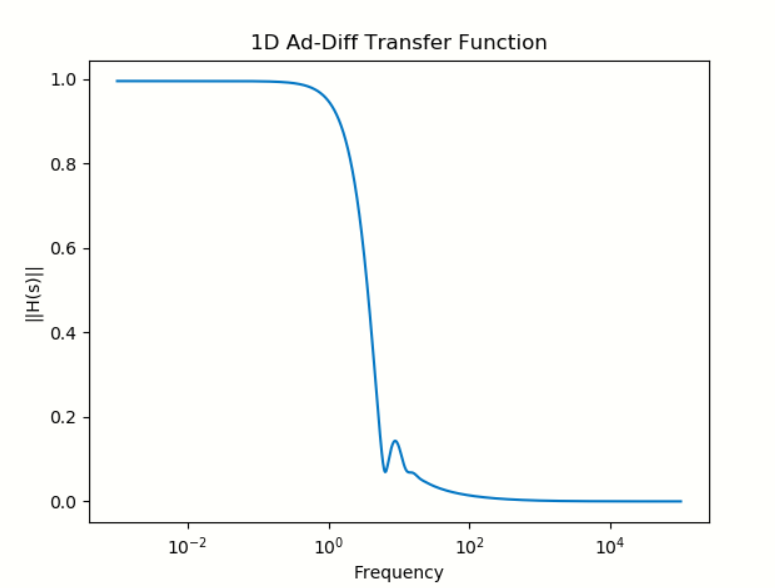
\includegraphics[width=7cm, height=5cm]{figures/1d_transfer.PNG}
\end{frame}
\section{Interpolatory Reduced Order Modeling}

\subsection{Projection Based ROM}

\begin{frame}{Projection Based ROM}
    To compute the reduced order model ${\bf \widehat{H}}(s)$, need to compute projection matrices ${\bf V}, {\bf W} \in \real^{n \times r}$ with $r << n$ such that:
\begin{align*}
    {\bf \widehat{A} } & = {\bf W^{T}} {\bf A} {\bf V} \\
    {\bf \widehat{b} } & = {\bf W^{T}} {\bf b} \\
    {\bf \widehat{c}}^T & = {\bf c}^T {\bf V} \\
    {\bf \widehat{E} } & = {\bf W^{T}} {\bf E} {\bf V}\\
    {\bf \widehat{H}}(s) & = {\bf \widehat{c}}^T \big( s{\bf \widehat{E}}-{\bf \widehat{A}} \big)^{-1} {\bf \widehat{b}} + {\bf \widehat{d}} 
\end{align*}
\\
Given a set of training frequencies $\{\sigma_1, \dots \sigma_r\} \subset \mathbb{I}$, want to find ${\bf V}, {\bf W}$ such that ${\bf H}(\sigma) = {\bf \widehat H}(\sigma)$ for all the training frequencies\\
\bigskip
How to compute ${\bf V}$ and ${\bf W}$?
    
\end{frame}
%%%%%%%%%%%%%%%%%%%%%%%%%%%%%%%%%%%%%%%%%%%%%%%%%%%%%%%%%%%%%%%%%%%%%%
\begin{frame}{Projection Based ROM}
\begin{theorem}
Let \(\sigma \in \mathbb{C}\) be such that \(\big(\sigma{\bf E}-{\bf A} \big)\) and \(\big(\sigma{\bf \widehat E}-{\bf \widehat A} \big)\) are non-singular. Also, let \({\bf V},{\bf W} \in \mathbb{C}^{n \times r}\) have full rank. Then,\\
\bigskip
\begin{enumerate}
    \item <1-> If \(\big( \sigma{\bf E}-{\bf A} \big)^{-1}{\bf b} \in \mathcal{R}\big({\bf V}\big) \), then \({\bf H}(\sigma) = {\bf \widehat{H}}(\sigma)\)
    \item <1-> If \(\big( \sigma{\bf E}^T-{\bf A}^T \big)^{-1} {\bf c} \in \mathcal{R}\big({\bf W}\big) \), then \({\bf H}(\sigma) = {\bf \widehat{H}}(\sigma)\)
    \item If (1) and (2) hold, then \({\bf H}'(\sigma) = {\bf \widehat H}'(\sigma)\)
\end{enumerate}

\end{theorem} 
\noindent

\end{frame}
%%%%%%%%%%%%%%%%%%%%%%%%%%%%%%%%%%%%%%%%%%%%%%%%%%%%%%%%%%%%%%%%

\begin{frame}{Proof of Interpolation Property}

Assume \(\big( \sigma{\bf E}-{\bf A} \big)^{-1}{\bf b} \in \mathcal{R}\big({\bf V}\big) \)\\

\bigskip

Define:
\begin{align*}
    \mathbb{P}(s) & = {\bf V} \Big( s{\bf E-A} \Big)^{-1} {\bf W^{T}} \Big( s{\bf E-A} \Big)\\
    \mathbb{Q}(s) & = \Big( s{\bf E-A} \Big) {\bf V} \Big( s{\bf E-A} \Big)^{-1} {\bf W^{T}}
\end{align*}
\\
\bigskip
\(\mathbb{P}(s)^2 =\mathbb{P}(s)\) and \(\mathbb{Q}(s)^2 = \mathbb{Q}(s) \implies \mathbb{P}(s)\) and \(\mathbb{Q}(s)\) are projections.
\\
\bigskip
Also, make note that \( \mathcal{R}\big( {\bf V} \big) =  \mathcal{R}\big( \mathbb{P}(\sigma) \big)  \) and \(\mathcal{R}\big({\bf W}\big) = \mathcal{R}\big({\bf I - \mathbb{Q}(\sigma)}\big) \).

\end{frame}

%%%%%%%%%%%%%%%%%%%%%%%%%%%%%%%%%%%%%%%%%%%%%%%%%%%%%%%%%%%%%%%%%%%%%%%%%%%%%%%%%%%%%%%%%%%%%%%%%%%%%%%%%%%%%%%%%%

\begin{frame}{Proof of Interpolation Property}
Consider the identity:
$$
    {\bf H}(s) -{\bf \widehat{H}}(s) = 
    {\bf c}^T \Big( s{\bf E-A} \Big)^{-1} \Big( {\bf I} - \mathbb{Q}(s) \Big) \Big( s{\bf E-A} \Big) \Big( {\bf I} - \mathbb{P}(s) \Big) \Big( s{\bf E-A} \Big)^{-1} {\bf b}
$$
\\


Evaluate at \(\sigma\), to get:
$$
    {\bf H}(s) -{\bf \widehat{H}}(s) = \dots \Big( {\bf I} - \mathbb{P}(\sigma)\Big) \Big( \sigma {\bf E-A} \Big)^{-1} {\bf b}
$$
\\
By assumption, \(\Big( \sigma {\bf E-A} \Big)^{-1} {\bf b} \in \mathcal{R}\big({\bf V}\big) \) or \( \in \mathcal{N}\big( {\bf I} - \mathbb{P}(\sigma) \big)\)\\
\bigskip
So:
$$ {\bf H}(\sigma) -{\bf \widehat{H}}(\sigma)  = 0 \implies {\bf H}(\sigma)  = {\bf \widehat{H}}(\sigma)
$$\\
\bigskip
Proof of part (2) follows similarly.    
\end{frame}

%%%%%%%%%%%%%%%%%%%%%%%%%%%%%%%%%%%%%%%%%%%%%%%%%%
\begin{frame}{Proof of Interpolation Property}

Assume parts (1) and (2) of the theorem hold\\

\bigskip

Consider the identity from before:
$$
    {\bf H}(s) -{\bf \widehat{H}}(s) = 
    {\bf c}^T \Big( s{\bf E-A} \Big)^{-1} \Big( {\bf I} - \mathbb{Q}(s) \Big) \Big( s{\bf E-A} \Big) \Big( {\bf I} - \mathbb{P}(s) \Big) \Big( s{\bf E-A} \Big)^{-1} {\bf b}
$$

Evaluate at $s = \sigma + \epsilon$:

$${\bf H}(\sigma + \epsilon) -{\bf \widehat{H}}(\sigma + \epsilon) = \mathcal{O}(\epsilon^2)$$

Since ${\bf H}(\sigma) = {\bf \widehat H}(\sigma)$ by the assumption,

$$\lim_{\epsilon \to 0} \frac{1}{\epsilon}\Big({\bf H}(\sigma + \epsilon) - {\bf H}(\sigma)\Big) - \frac{1}{\epsilon}\Big({\bf \widehat H}(\sigma + \epsilon) - {\bf \widehat H}(\sigma)\Big) = 0$$
which proves part (3) of the theorem.
\end{frame}
%%%%%%%%%%%%%%%%%%%%%%%%%%%%%%%%%%%%%%%%%%%%
\begin{frame}{Projection Matrix Generation}
Choose a list of interpolation frequencies, \([\sigma_1,\sigma_2, ... , \sigma_r]\).\\
\bigskip
Then let us construct the projection matrices and as follows:
\begin{align*}
    {\bf V} & = \Big[ \big( \sigma_1{\bf E}-{\bf A} \big)^{-1}{\bf b}, \dots, \big( \sigma_r{\bf I}-{\bf A} \big)^{-1}{\bf E} \Big] \\
    {\bf W} & = \Big[ \big( \sigma_1{\bf E}^T-{\bf A}^T \big)^{-1} {\bf c}, \dots, \big( \sigma_r{\bf E}^T-{\bf A}^T \big)^{-1} {\bf c} \Big] \\ 
\end{align*}
\end{frame}
%%%%%%%%%%%%%%%%%%%%%%%%%%%%%%%%%%%%%%%%%%%%%%%%%%%%%%%%%%%%%%%%%%%%%%%%%%%%%%%%%%%%%%%%%%%%%%%%%%%%
\begin{frame}{Projection ROM Performance}
\centering
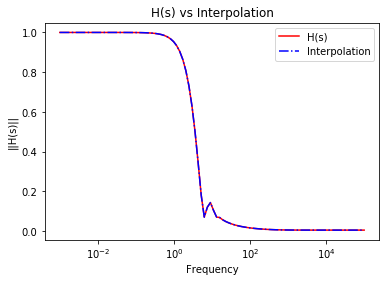
\includegraphics[width=5cm, height= 4cm]{1D_proj.png}
\bigskip
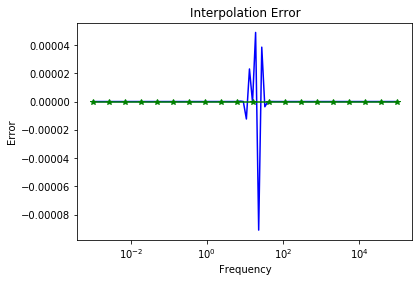
\includegraphics[width=5cm, height=4cm]{1D_proj_err.png}
    
\end{frame}
%%%%%%%%%%%%%%%%%%%%%%%%%%%%%%%%%%%%%%%
\begin{frame}{Projection ROM: Complex to Real}
Since \(\sigma_j\) is complex, \({\bf V}\) and \({\bf W} \in \mathbb{C}\).
\\
The original problem is in the time domain.
\bigskip
\begin{itemize}
    \item <1->Need  real matrices $\bf \widehat A$, $\bf \widehat b$, $\bf \widehat c$, $\bf \widehat d$, and $\bf \widehat E$ \\
    \item <1-> To get \({\bf A} \in \real^{n \times n}, {\bf b} \in \real^{n}\), etc., need real valued {\bf V},{\bf W}
\end{itemize}
\bigskip
\begin{itemize}
    \item <1-> Problem:
    \begin{itemize}
        \item How do we retain the info in {\bf V},{\bf W}?
    \end{itemize}
\end{itemize}
\bigskip
Split into their real and imaginary parts?
\end{frame}



%%%%%%%%%%%%%%%%%%%%%%%%%%%%%%%%%%%%%%%

\begin{frame}{Projection ROM: Complex to Real}
\begin{itemize}
    \item <1-> Split into real and imaginary parts:
\end{itemize}
 Let $\mathbf{V} = \mathbf{V_a} + i \mathbf{V_b}$ and $\mathbf W = \mathbf W_a + i \mathbf W_b$.
\\
\bigskip
Choose $\bf V_{real} = \left[V_a V_b\right]$ and $\bf W_{real} = \left[W_a W_b\right]$.
\\
\bigskip

\begin{itemize}
    \item Problem:
    \begin{itemize}
        \item {\bf V},{\bf W} may be singular
    \end{itemize}
\end{itemize}
\bigskip
Solution? SVD!
\end{frame}
%%%%%%%%%%%%%%%%%%%%%%%%%%%%55
\begin{frame}{Projection ROM: Complex to Real}
SVD purpose = 
\begin{itemize}
    \item <1->remove dependent information
    \item <1-> ensure non-singularity of \( \Big( \sigma \widehat{{\bf E}} - \widehat{{\bf A}} \Big) \)
\end{itemize}

\bigskip
Let $\bf U_v \Sigma_v V_v^T = \left[V_a V_b\right]$ and $\bf U_w \Sigma_w V_w^T = \left[W_a W_b\right]$.
\\
\bigskip
Given a tolerance for the normalized singular values, let \(k_v, k_w =\) number of normalized singular values \(>\) the tolerance.
\bigskip
Set k = max(\(k_v, k_w\)).\\
\bigskip
Then \({\bf V_{real}} = {\bf U_{v_k}}\) and \({\bf W_{real}} = {\bf U_{w_k}}\)
\end{frame}


\subsection{Loewner Framework ROM}

\begin{frame}{Loewner Method Motivation}
The projection based ROM works very well, as proven by the error plot. What do we need the Loewner Method for?\\
\bigskip
Reasons:
\begin{itemize}
    \item To use the projection method, need {\bf A},{\bf b},{\bf c},{\bf d}, and {\bf E}
    \item In some applications, matrices not given
    \item Can be used with only transfer function data
    \item Retains interpolation property, mimics projection method
\end{itemize}
\bigskip
Downsides:
\begin{itemize}
    \item Loewner matrices might become singular if too many sample frequencies are used
    \item Which frequencies to sample data from?
    \item Needs {\bf d} in FOM
\end{itemize}
    
\end{frame}

%%%%%%%%%%%%%%%%%%%%%%%%%%%%%
\begin{frame}{Loewner Data Setup}
First, lets assume that in the FOM ${\bf d} =0$\\
\bigskip
Left frequencies:
\begin{align*}
    {\bf \Sigma} &= \{\sigma_1, \dots, \sigma_r\} \subset \mathbb{I}
\end{align*}
\\
Right frequencies:
\begin{align*}
    {\bf \Theta} &= \{\theta_1, \dots, \theta_r\} \subset \mathbb{I}
\end{align*}

with

$${\bf \Sigma} \cap {\bf \Theta} = \emptyset$$

\end{frame}
%%%%%%%%%%%%%%%%%%%%%%%%%%%%%%%%%%%%%%%%%%%%%%%%%%%%%%%%%%%%%%%%%%%%%%%%%%%%%%%%%%%%%%
\begin{frame}{Loewner Matrices and ROM}

Construct the Loewner Matrix:
\begin{align*}
    \mathbb{L}_{ij} &=  \frac{{\bf H}(\sigma_i)-{\bf H}(\theta_j)}{\sigma_i - \theta_j}\\
\end{align*}
Construct the Shifted Loewner Matrix:
\begin{align*}
    \mathbb{M}_{ij} &= \frac{\sigma_i{\bf H}(\sigma_i)-\theta_j{\bf H}(\theta_j)}{\sigma_i - \theta_j}\\
\end{align*}

\end{frame}
%%%%%%%%%%%%%%%%%%%%%%%%%%%%%%%%%%%%%%%%%%%%%%%%%%%%%%%%%%%%%%%%%%%%%%%%%%%%%%%%%%%%%%
\begin{frame}{Loewner Matrices and ROM}
Construct the Loewner ROM:

\begin{align*}
    {\bf \widehat{A} } & = -\mathbb{M} \\
    {\bf \widehat{b} } & = \left[{\bf H}(\sigma_1), \dots, {\bf H}(\sigma_r) \right]^T\\
    {\bf \widehat{c}}^T & = \left[{\bf H}(\theta_1), \dots, {\bf H}(\theta_r) \right]\\
    {\bf \widehat{E} } & = -\mathbb{L}\\
    {\bf \widehat{d} } & = 0 \\ \\
    {\bf \widehat{H}}(s) & = {\bf \widehat{c}}^T \big( s{\bf \widehat{E}}-{\bf \widehat{A}} \big)^{-1} {\bf \widehat{b}} + {\bf \widehat{d}}
\end{align*}


\end{frame}

%%%%%%%%%%%%%%%%%%%%%%%%%%%%%%%%%%%%%%%%%%%%%%%%%%%%%

\begin{frame}{Loewner Interpolation Theorem}

\begin{theorem}
Assume $\mathbb{M}-s\mathbb{L}$ is invertible for all $s \in \Sigma \cup \Theta$.\\
\bigskip
Then, the previously described ROM transfer function interpolates at the left and right training frequencies:\\
\bigskip
${\bf H}(s) = {\bf \widehat H}(s)$ for all $s \in \Sigma \cup \Theta$
\end{theorem}

\end{frame}
%%%%%%%%%%%%%%%%%%%%%%%%%%%%%%%%%%%%%%%%%%%%%%%%%%%%%%%%%%
\begin{frame}{Loewner Interpolation Property Proof}

Simplify the constructed Loewner ROM 
\begin{align*}
{\bf \widehat{H}}(s) & = {\bf \widehat{c}}^T \big( s{\bf \widehat{E}}-{\bf \widehat{A}} \big)^{-1} {\bf \widehat{b}} \\
{\bf \widehat{H}}(s) &= \left[{\bf H}(\theta_1), \dots, {\bf H}(\theta_r) \right](\mathbb{M} - s \mathbb{L})^{-1} \left[{\bf H}(\sigma_1), \dots, {\bf H}(\sigma_r) \right]^T
\end{align*}

Consider the matrix $\mathbb{M} - s \mathbb{L}$ where $s \in \mathbb{C}$.\\
\bigskip
$$(\mathbb{M} - s \mathbb{L})_{i,j} = \frac{s - \theta_j}{\sigma_i - \theta_j}{\bf H}(\theta_j) + \frac{\sigma_i - s}{\sigma_i - \theta_j}{\bf H}(\sigma_i)$$\\

\bigskip

Two interpolatory cases for s:

\begin{enumerate}
    \item $s = \theta_k$ for some k
    \item $s = \sigma_k$ for some k
\end{enumerate}

\end{frame}

%%%%%%%%%%%%%%%%%%%%%%%%%%%%%%%%%%%%%%%%%%%%%%
\begin{frame}{Loewner Interpolation Property Proof}

Consider case where $s = \theta_k$.\\
\bigskip
Recall:
$$(\mathbb{M} - s \mathbb{L})_{i,j} = \frac{s - \theta_j}{\sigma_i - \theta_j}{\bf H}(\theta_j) + \frac{\sigma_i - s}{\sigma_i - \theta_j}{\bf H}(\sigma_i)$$

\begin{center}
$(\mathbb{M} - \theta_k \mathbb{L})e_k = \left[{\bf H}(\sigma_1), \dots, {\bf H}(\sigma_r) \right]^T \implies$ \\
$e_k = (\mathbb{M} - \theta_k \mathbb{L})^{-1}\left[{\bf H}(\sigma_1), \dots, {\bf H}(\sigma_r) \right]^T$
\end{center}

\begin{center}
$\left[{\bf H}(\theta_1), \dots, {\bf H}(\theta_r) \right] e_k = {\bf H}(\theta_k)$\\

$\left[{\bf H}(\theta_1), \dots, {\bf H}(\theta_r) \right] (\mathbb{M} - \theta_k \mathbb{L})^{-1}\left[{\bf H}(\sigma_1), \dots, {\bf H}(\sigma_r) \right]^T = {\bf \widehat H}(\theta_k)$
\end{center}

Therefore, ${\bf H}(\theta_k) = {\bf \widehat H}(\theta_k)$

\end{frame}
%%%%%%%%%%%%%%%%%%%%%%%%%%%%%%%%%%%%%%%%%%%%%%%%%%%%%%%%%%%
\begin{frame}{Loewner Interpolation Property Proof}

Consider case where $s = \sigma_k$.\\
\bigskip
Recall:
$$(\mathbb{M} - s \mathbb{L})_{i,j} = \frac{s - \theta_j}{\sigma_i - \theta_j}{\bf H}(\theta_j) + \frac{\sigma_i - s}{\sigma_i - \theta_j}{\bf H}(\sigma_i)$$


\begin{center}
$e_k^T(\mathbb{M} - \sigma_k \mathbb{L}) = \left[{\bf H}(\theta_1), \dots, {\bf H}(\theta_r) \right] \implies$ \\
$e_k^T = \left[{\bf H}(\theta_1), \dots, {\bf H}(\theta_r) \right] (\mathbb{M} - \sigma_k \mathbb{L})^{-1}$
\end{center}

\begin{center}
$e_k^T \left[{\bf H}(\sigma_1), \dots, {\bf H}(\sigma_r) \right]^T = {\bf H}(\sigma_k)$\\

$\left[{\bf H}(\theta_1), \dots, {\bf H}(\theta_r) \right] (\mathbb{M} - \sigma_k \mathbb{L})^{-1}\left[{\bf H}(\sigma_1), \dots, {\bf H}(\sigma_r) \right]^T = {\bf \widehat H}(\sigma_k)$
\end{center}

Therefore, ${\bf H}(\sigma_k) = {\bf \widehat H}(\sigma_k)$

\end{frame}

%%%%%%%%%%%%%%%%%%%%%%%%%%%%%%%%%%%%%%%%%%%%%%%%%%%%%%%%%%%%%%%%
\begin{frame}{Dealing with Singular Loewner Matrices}

Necessary that Loewner matrices are nonsingular\\

\bigskip

\begin{itemize}
    \item More frequencies leads to singular Loewner matrices
    \item ROM transfer function will be undefined 
\end{itemize}

\bigskip
Use SVD to extract independent columns of matrices:
\\
\begin{align*}
\bf U_1 \Sigma_1 V_1^* &= \left[ \mathbb{L} \; \mathbb{M} \right] \\
\bf U_2 \Sigma_2 V_2^* &= \left[ \mathbb{L} \; \mathbb{M} \right]^T 
\end{align*}

Given a tolerance for the normalized singular values, let \(k_1, k_2 =\) number of normalized singular values \(>\) the tolerance. Set k = max(\(k_v, k_w\)).\\
\bigskip
Let $\bf U = U_{1k}$ and $\bf V = V_{2k}$.
\end{frame}

%%%%%%%%%%%%%%%%%%%%%%%%%%%%%%%%%%%%%%%%%%%%%%%%%%%%%%%%%%%%%%%%

\begin{frame}{Dealing with Singular Loewner Matrices}

Construct the new Loewner ROM as:

\begin{align*}
    {\bf \widehat{A} } & = {\bf-U^*\mathbb{M}V}\\
    {\bf \widehat{b} } & = {\bf U^*} \left[{\bf H}(\sigma_1), \dots, {\bf H}(\sigma_r) \right]^T\\
    {\bf \widehat{c}}^T & = \left[{\bf H}(\theta_1), \dots, {\bf H}(\theta_r) \right]{\bf V} \\
    {\bf \widehat{E} } & = {\bf -U^*\mathbb{L} V}\\
    {\bf \widehat{d} } & = 0 \\ \\
    {\bf \widehat{H}}(s) & = {\bf \widehat{c}}^T \big( s{\bf \widehat{E}}-{\bf \widehat{A}} \big)^{-1} {\bf \widehat{b}} + {\bf \widehat{d}}
\end{align*}
    
Interpolatory properties of the new Loewner ROM are beyond the scope of this presentation    
\end{frame}
%%%%%%%%%%%%%%%%%%%%%%%%%%%%%%%%%%%%%%%%%%%%%%%%%%
\begin{frame}{Lowner Framework Implementation}

\begin{enumerate}
    \item Choose disjoint imaginary left and right frequencies $\{\sigma_1, \dots, \sigma_r\}$ and $\{\theta_1, \dots, \theta_r\}$, respectively
    \item Compute $\mathbb{L}$ and $\mathbb{M}$
    \begin{itemize}
        \item $\mathbb{L}_{ij} =  \frac{{\bf H}(\sigma_i)-{\bf H}(\theta_j)}{\sigma_i - \theta_j}$
        \item $\mathbb{M}_{ij} = \frac{\sigma_i{\bf H}(\sigma_i)-\theta_j{\bf H}(\theta_j)}{\sigma_i - \theta_j}$
    \end{itemize}
    \item Compute $\bf U$ and $\bf V$ from the SVD of the Loewner pencils
    \item Use the Loewner matrices, $\bf U$, $\bf V$, and the left and right transfer function data to compute the ROM  
\end{enumerate}


\end{frame}
%%%%%%%%%%%%%%%%%%%%%%%%%%%%%%%%%%%%%%%%%%%%%%%%%%%%%%%%%%%%%%%%
\begin{frame}{Actual H(s) vs Loewner H(s)}

Using 5 left and 5 right frequencies:

\centering
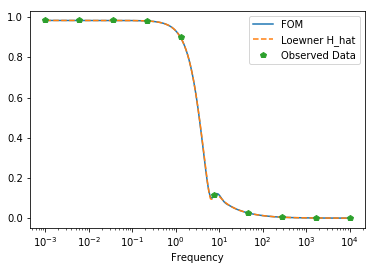
\includegraphics[width=5cm, height= 4cm]{figures/loewner2.png}
\bigskip
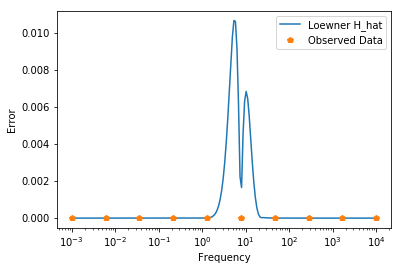
\includegraphics[width=5cm, height=4cm]{figures/loewner1.png}

\end{frame}
%%%%%%%%%%%%%%%%%%%%%%%%%%%%%%%%%%%%%%%%%%
\begin{frame}{Converting Loewner to Real}

Since the right and left frequencies are complex, the ouput of the transfer function at these frequencies will be complex as well. This leads to complex Loewner matrices.\\
\bigskip
The original problem is in the time domain.\\
\bigskip
\begin{itemize}
    \item <1-> Need real matrices $\bf \widehat A$, $\bf \widehat b$, $\bf \widehat c$, $\bf \widehat d$, and $\bf \widehat E$\\
\end{itemize}
\bigskip
Compute real $\mathbb{L}$ and $\mathbb{M}$
\bigskip
\begin{itemize}
    \item <1-> Problem:
    \begin{itemize}
        \item How do we retain the info in $\mathbb{L}$, $\mathbb{M}$?
    \end{itemize}
\end{itemize}
\bigskip
Utilize the fact that $\overline{\bf{H}(s)} = \bf{H}(\overline{s})$.

\end{frame}

%%%%%%%%%%%%%%%%%%%%%%%%%%%%%%%%%%%%%%%%%%%%%%%%%%
\begin{frame}{Converting Loewner to Real}

First include the complex conjugate data in the setup.\\
\bigskip
Left frequencies:
\begin{align*}
    {\bf \Sigma} &= \{\sigma_1, \dots, \sigma_{2r}\} \subset \mathbb{I}
\end{align*}
where $\sigma_{2i} = \overline \sigma_{2i-1}$\\
\bigskip
Right frequencies:
\begin{align*}
    {\bf \Theta} &= \{\theta_1, \dots, \theta_{2r}\} \subset \mathbb{I}
\end{align*}
where $\theta_{2i} = \overline \theta_{2i-1}$\\

\end{frame}
%%%%%%%%%%%%%%%%%%%%%%%%%%%%%%%%%%%%%%%%%%%%%%%%%%
\begin{frame}{Converting Loewner to Real}

Let ${\bf J} \in \mathbb{C}^{n \times n}$ be a block diagonal matrix with $\frac{1}{\sqrt 2}\begin{bmatrix} 1 & -i\\ 1 & i\end{bmatrix}$ repeated on the diagonal.\\
\bigskip
Use the following real Loewner matrices to compute ${\bf U}_R$ and ${\bf V}_R$:
\begin{align*}
    \mathbb{L}_R &= {\bf J}^* \mathbb{L} {\bf J}\\
    \mathbb{M}_R &= {\bf J}^* \mathbb{M} {\bf J}\\
\end{align*}


\end{frame}
%%%%%%%%%%%%%%%%%%%%%%%%%%%%%%%%%%%%%%%%%%%%%
\begin{frame}{Converting Loewner to Real}

Construct the real Loewner ROM as:

\begin{align*}
    {\bf \widehat{A} } & = -{\bf U}_R^T \mathbb{M}_R {\bf V}_R\\
    {\bf \widehat{b} } & = {\bf U}^T {\bf J}^* \left[{\bf H}(\sigma_1), \dots, {\bf H}(\sigma_r) \right]^T\\
    {\bf \widehat{c}}^T & = \left[{\bf H}(\theta_1), \dots, {\bf H}(\theta_r) \right] {\bf J} {\bf V} \\
    {\bf \widehat{E} } & = -{\bf U}_R^T \mathbb{L}_R {\bf V}_R\\
    {\bf \widehat{d} } & = 0 \\ \\
    {\bf \widehat{H}}(s) & = {\bf \widehat{c}}^T \big( s{\bf \widehat{E}}-{\bf \widehat{A}} \big)^{-1} {\bf \widehat{b}} + {\bf \widehat{d}}
\end{align*}

\end{frame}
%%%%%%%%%%%%%%%%%%%%%%%%%%%%%%%%%%%%%%%
\begin{frame}{How does this work?}

Consider computing $\mathbb{L}_R$ in the case where $\Sigma = \{\sigma, \overline \sigma\}$ and $\Theta = \{\theta, \overline \theta\}$:\\
\begin{align*}
\mathbb{L}_R &= \frac{1}{2} \begin{bmatrix} 1 & 1\\ i & -i \end{bmatrix}
\begin{bmatrix} \frac{{\bf H}(\sigma) - {\bf H}(\theta)}{\sigma - \theta} & \frac{\overline{{\bf H}(\sigma)} - {\bf H}(\theta)}{\overline \sigma - \theta}\\[1em] \frac{{\bf H}(\sigma) - \overline{{\bf H}(\theta)}}{\sigma - \overline \theta} & \frac{\overline{{\bf H}(\sigma)} - \overline{{\bf H}(\theta)}}{\overline \sigma - \overline \theta} \end{bmatrix}
\begin{bmatrix} 1 & -i\\ 1 & i\end{bmatrix}\\[1em]
\mathbb{L}_R &= \begin{bmatrix} re(\frac{{\bf H}(\sigma) - {\bf H}(\theta)}{\sigma - \theta}) & im(\frac{{\bf H}(\sigma) - {\bf H}(\theta)}{\sigma - \theta}) \\[1em] -im(\frac{{\bf H}(\sigma) - {\bf H}(\theta)}{\sigma - \theta}) & re(\frac{{\bf H}(\sigma) - {\bf H}(\theta)}{\sigma - \theta})\end{bmatrix}
\end{align*}

The matrix $\mathbb{L}_R$ is real but encapsulates the same information as the complex number $\frac{{\bf H}(\sigma) - {\bf H}(\theta)}{\sigma - \theta}$.\\
\bigskip
Same holds for $\mathbb{M}_R$.
\end{frame}
\subsection{Method Comparison}

\begin{frame}{Comparison of Methods}
\begin{itemize}
\item 10 training frequencies logarithmically spaced between $10^{-3}$ and $10^4$\\
\item Tolerance of $10^{-12}$ for cutting off SVD's
in both methods\\
\bigskip
\item Size of ROMs: \\
\begin{itemize}
    \item Loewner Framework - 5 by 5
    \item Projection - 10 by 10
\end{itemize}
\end{itemize}

\centering
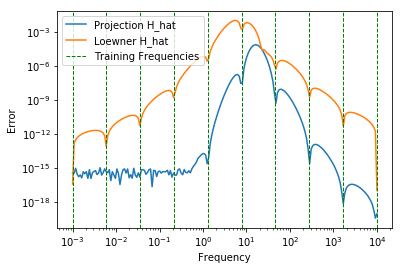
\includegraphics[width=7.5cm, height= 6cm]{figures/comparison0.png}

\end{frame}
%%%%%%%%%%%%%%%%%%%%%%%%%%%%%%%%%%%%%%%%%%%%%%%%
\begin{frame}{Comparison of Methods}
\begin{itemize}
    \item Covert both ROMs to real domain\\
    \bigskip
    \item Size of ROMs: \\
    \begin{itemize}
        \item Loewner Framework - 8 by 8
        \item Projection - 15 by 15
    \end{itemize}
\end{itemize}

\centering
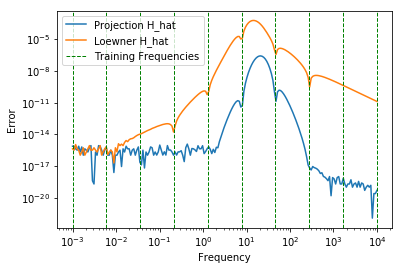
\includegraphics[width=7.5cm, height= 6cm]{figures/comparison1.png}
\end{frame}
%%%%%%%%%%%%%%%%%%%%%%%%%%%%%%%%%%%%%%%%%%%

\begin{frame}{Comparison of Methods}
Compare ROM methods to the FOM in the time domain:\\
\bigskip
\begin{center}
 Let $u(t) = sin(2 \pi t)$, for $0 \leq t \leq 0.5$   
\end{center}

\centering
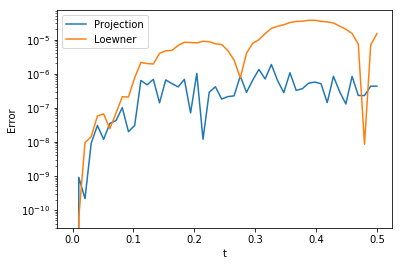
\includegraphics[width=7.5cm, height= 6cm]{figures/comparison2.png}
\end{frame}

\section{Further Research}

\begin{frame}{Further Research}
\begin{itemize}
    \item Loewner with noise
    \begin{itemize}
        \item In most data collection, there is error. In our experiments, noise \(\implies\) large error. Error correction techniques may be necessary to develop.
    \end{itemize}
    \bigskip
    \item Generalized eigenvalue problem and error spikes
    \begin{itemize}
        \item Closely related to the first problem. With noise, the eigenvalues shift closer to the imaginary axis, causing problems. As a result the Loewner matrices become singular.
    \end{itemize}
    \bigskip
    \item Performace optimization (Loewner Method)
    \begin{itemize}
        \item It would be interesting to explore optimal selection of frequencies and other related factors that could influence results.
    \end{itemize}
\end{itemize}





\end{frame}
\section{Resources}

\begin{frame}

\frametitle{Resources}

[1] A.C. Antoulas, C. Beattie, S. Gugercin, {\it{Interpolatory Methods for Model Reduction}}, pg. 33-85, June 14, 2019\\
\bigskip
[2] M. Heinkenschloss, a big thanks for mentoring this project!\\

\end{frame} 


\end{document}